\documentclass{standalone}
\usepackage{tikz}
\usetikzlibrary{patterns, positioning}


\begin{document}
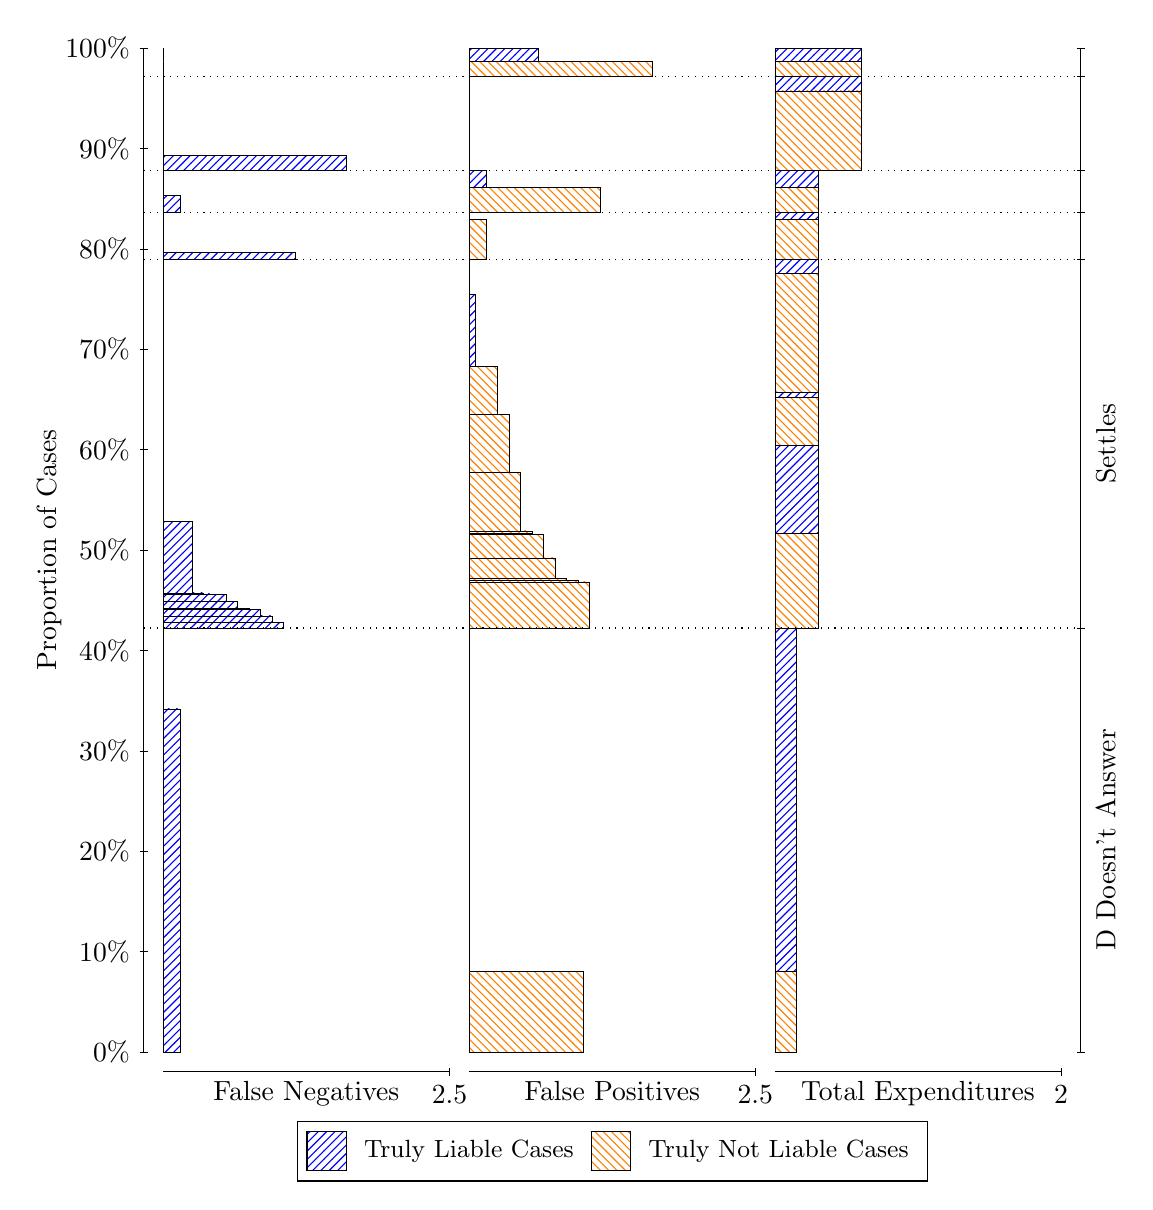
\begin{tikzpicture}
\draw[black, very thin] (1.5,1.75) -- (1.5,14.5);
\node[rotate=90, text=black, anchor=center] at (0.3, 8.125) {Proportion of Cases};
\draw[black, very thin] (1.45,1.75) -- (1.55,1.75);
\node[text=black, anchor=east] at (1.45, 1.75) {0\%};
\draw[black, very thin] (1.45,3.025) -- (1.55,3.025);
\node[text=black, anchor=east] at (1.45, 3.025) {10\%};
\draw[black, very thin] (1.45,4.3) -- (1.55,4.3);
\node[text=black, anchor=east] at (1.45, 4.3) {20\%};
\draw[black, very thin] (1.45,5.575) -- (1.55,5.575);
\node[text=black, anchor=east] at (1.45, 5.575) {30\%};
\draw[black, very thin] (1.45,6.85) -- (1.55,6.85);
\node[text=black, anchor=east] at (1.45, 6.85) {40\%};
\draw[black, very thin] (1.45,8.125) -- (1.55,8.125);
\node[text=black, anchor=east] at (1.45, 8.125) {50\%};
\draw[black, very thin] (1.45,9.4) -- (1.55,9.4);
\node[text=black, anchor=east] at (1.45, 9.4) {60\%};
\draw[black, very thin] (1.45,10.675) -- (1.55,10.675);
\node[text=black, anchor=east] at (1.45, 10.675) {70\%};
\draw[black, very thin] (1.45,11.95) -- (1.55,11.95);
\node[text=black, anchor=east] at (1.45, 11.95) {80\%};
\draw[black, very thin] (1.45,13.225) -- (1.55,13.225);
\node[text=black, anchor=east] at (1.45, 13.225) {90\%};
\draw[black, very thin] (1.45,14.5) -- (1.55,14.5);
\node[text=black, anchor=east] at (1.45, 14.5) {100\%};

\draw[black, very thin] (13.4,1.75) -- (13.4,14.5);
\draw[black, very thin] (13.35,1.75) -- (13.45,1.75);
\node[anchor=west] at (13.35, 1.75) {};
\draw[black, very thin] (13.35,7.1342) -- (13.45,7.1342);
\node[anchor=west] at (13.35, 7.1342) {};
\draw[black, very thin] (13.35,11.813) -- (13.45,11.813);
\node[anchor=west] at (13.35, 11.813) {};
\draw[black, very thin] (13.35,12.411) -- (13.45,12.411);
\node[anchor=west] at (13.35, 12.411) {};
\draw[black, very thin] (13.35,12.945) -- (13.45,12.945);
\node[anchor=west] at (13.35, 12.945) {};
\draw[black, very thin] (13.35,14.143) -- (13.45,14.143);
\node[anchor=west] at (13.35, 14.143) {};
\draw[black, very thin] (13.35,14.5) -- (13.45,14.5);
\node[anchor=west] at (13.35, 14.5) {};

\draw[black, very thin, pattern color=blue, pattern=north east lines] (1.75,1.75) rectangle (1.968,6.1077);
\draw[black, very thin, pattern color=orange, pattern=north west lines] (1.75,6.1077) rectangle (1.75,7.1342);
\draw[black, very thin, pattern color=blue, pattern=north east lines] (1.75,7.1342) rectangle (3.276,7.2022);
\draw[black, very thin, pattern color=blue, pattern=north east lines] (1.75,7.2022) rectangle (3.1307,7.2889);
\draw[black, very thin, pattern color=blue, pattern=north east lines] (1.75,7.2889) rectangle (2.9853,7.3753);
\draw[black, very thin, pattern color=blue, pattern=north east lines] (1.75,7.3753) rectangle (2.84,7.3831);
\draw[black, very thin, pattern color=blue, pattern=north east lines] (1.75,7.3831) rectangle (2.6947,7.4743);
\draw[black, very thin, pattern color=blue, pattern=north east lines] (1.75,7.4743) rectangle (2.5493,7.5567);
\draw[black, very thin, pattern color=blue, pattern=north east lines] (1.75,7.5567) rectangle (2.404,7.569);
\draw[black, very thin, pattern color=blue, pattern=north east lines] (1.75,7.569) rectangle (2.2587,7.5808);
\draw[black, very thin, pattern color=blue, pattern=north east lines] (1.75,7.5808) rectangle (2.1133,8.4873);
\draw[black, very thin, pattern color=orange, pattern=north west lines] (1.75,8.4873) rectangle (1.75,11.813);
\draw[black, very thin, pattern color=blue, pattern=north east lines] (1.75,11.813) rectangle (3.4213,11.903);
\draw[black, very thin, pattern color=orange, pattern=north west lines] (1.75,11.903) rectangle (1.75,12.411);
\draw[black, very thin, pattern color=blue, pattern=north east lines] (1.75,12.411) rectangle (1.968,12.624);
\draw[black, very thin, pattern color=orange, pattern=north west lines] (1.75,12.624) rectangle (1.75,12.945);
\draw[black, very thin, pattern color=blue, pattern=north east lines] (1.75,12.945) rectangle (4.0753,13.133);
\draw[black, very thin, pattern color=orange, pattern=north west lines] (1.75,13.133) rectangle (1.75,14.143);
\draw[black, very thin, pattern color=orange, pattern=north west lines] (1.75,14.143) rectangle (1.75,14.326);
\draw[black, very thin, pattern color=blue, pattern=north east lines] (1.75,14.326) rectangle (1.75,14.5);
\draw[black, very thin, pattern color=orange, pattern=north west lines] (5.6333,1.75) rectangle (7.0867,2.7764);
\draw[black, very thin, pattern color=blue, pattern=north east lines] (5.6333,2.7764) rectangle (5.6333,7.1342);
\draw[black, very thin, pattern color=orange, pattern=north west lines] (5.6333,7.1342) rectangle (7.1593,7.7202);
\draw[black, very thin, pattern color=orange, pattern=north west lines] (5.6333,7.7202) rectangle (7.014,7.7419);
\draw[black, very thin, pattern color=orange, pattern=north west lines] (5.6333,7.7419) rectangle (6.8687,7.7653);
\draw[black, very thin, pattern color=orange, pattern=north west lines] (5.6333,7.7653) rectangle (6.7233,8.0252);
\draw[black, very thin, pattern color=orange, pattern=north west lines] (5.6333,8.0252) rectangle (6.578,8.3206);
\draw[black, very thin, pattern color=orange, pattern=north west lines] (5.6333,8.3206) rectangle (6.4327,8.3427);
\draw[black, very thin, pattern color=orange, pattern=north west lines] (5.6333,8.3427) rectangle (6.4327,8.3678);
\draw[black, very thin, pattern color=orange, pattern=north west lines] (5.6333,8.3678) rectangle (6.2873,9.1085);
\draw[black, very thin, pattern color=orange, pattern=north west lines] (5.6333,9.1085) rectangle (6.142,9.851);
\draw[black, very thin, pattern color=orange, pattern=north west lines] (5.6333,9.851) rectangle (5.9967,10.46);
\draw[black, very thin, pattern color=blue, pattern=north east lines] (5.6333,10.46) rectangle (5.706,11.367);
\draw[black, very thin, pattern color=blue, pattern=north east lines] (5.6333,11.367) rectangle (5.6333,11.813);
\draw[black, very thin, pattern color=orange, pattern=north west lines] (5.6333,11.813) rectangle (5.8513,12.321);
\draw[black, very thin, pattern color=blue, pattern=north east lines] (5.6333,12.321) rectangle (5.6333,12.411);
\draw[black, very thin, pattern color=orange, pattern=north west lines] (5.6333,12.411) rectangle (7.3047,12.733);
\draw[black, very thin, pattern color=blue, pattern=north east lines] (5.6333,12.733) rectangle (5.8513,12.945);
\draw[black, very thin, pattern color=orange, pattern=north west lines] (5.6333,12.945) rectangle (5.6333,13.955);
\draw[black, very thin, pattern color=blue, pattern=north east lines] (5.6333,13.955) rectangle (5.6333,14.143);
\draw[black, very thin, pattern color=orange, pattern=north west lines] (5.6333,14.143) rectangle (7.9587,14.326);
\draw[black, very thin, pattern color=blue, pattern=north east lines] (5.6333,14.326) rectangle (6.5053,14.5);
\draw[black, very thin, pattern color=orange, pattern=north west lines] (9.5167,1.75) rectangle (9.7892,2.7764);
\draw[black, very thin, pattern color=blue, pattern=north east lines] (9.5167,2.7764) rectangle (9.7892,7.1342);
\draw[black, very thin, pattern color=orange, pattern=north west lines] (9.5167,7.1342) rectangle (10.062,8.3427);
\draw[black, very thin, pattern color=blue, pattern=north east lines] (9.5167,8.3427) rectangle (10.062,9.4505);
\draw[black, very thin, pattern color=orange, pattern=north west lines] (9.5167,9.4505) rectangle (10.062,10.06);
\draw[black, very thin, pattern color=blue, pattern=north east lines] (9.5167,10.06) rectangle (10.062,10.128);
\draw[black, very thin, pattern color=orange, pattern=north west lines] (9.5167,10.128) rectangle (10.062,11.636);
\draw[black, very thin, pattern color=blue, pattern=north east lines] (9.5167,11.636) rectangle (10.062,11.813);
\draw[black, very thin, pattern color=orange, pattern=north west lines] (9.5167,11.813) rectangle (10.062,12.321);
\draw[black, very thin, pattern color=blue, pattern=north east lines] (9.5167,12.321) rectangle (10.062,12.411);
\draw[black, very thin, pattern color=orange, pattern=north west lines] (9.5167,12.411) rectangle (10.062,12.733);
\draw[black, very thin, pattern color=blue, pattern=north east lines] (9.5167,12.733) rectangle (10.062,12.945);
\draw[black, very thin, pattern color=orange, pattern=north west lines] (9.5167,12.945) rectangle (10.607,13.955);
\draw[black, very thin, pattern color=blue, pattern=north east lines] (9.5167,13.955) rectangle (10.607,14.143);
\draw[black, very thin, pattern color=orange, pattern=north west lines] (9.5167,14.143) rectangle (10.607,14.326);
\draw[black, very thin, pattern color=blue, pattern=north east lines] (9.5167,14.326) rectangle (10.607,14.5);
\draw[black, dotted] (1.5,7.1342) -- (13.4,7.1342);
\draw[black, dotted] (1.5,11.813) -- (13.4,11.813);
\draw[black, dotted] (1.5,12.411) -- (13.4,12.411);
\draw[black, dotted] (1.5,12.945) -- (13.4,12.945);
\draw[black, dotted] (1.5,14.143) -- (13.4,14.143);
\draw[black, very thin] (1.75,1.5) -- (5.3833,1.5);
\node[text=black, anchor=north] at (3.5667, 1.5) {False Negatives};
\draw[black, very thin] (5.3833,1.45) -- (5.3833,1.55);
\node[text=black, anchor=north] at (5.3833, 1.45) {2.5};

\draw[black, very thin] (5.6333,1.5) -- (9.2667,1.5);
\node[text=black, anchor=north] at (7.45, 1.5) {False Positives};
\draw[black, very thin] (9.2667,1.45) -- (9.2667,1.55);
\node[text=black, anchor=north] at (9.2667, 1.45) {2.5};

\draw[black, very thin] (9.5167,1.5) -- (13.15,1.5);
\node[text=black, anchor=north] at (11.333, 1.5) {Total Expenditures};
\draw[black, very thin] (13.15,1.45) -- (13.15,1.55);
\node[text=black, anchor=north] at (13.15, 1.45) {2};

\node[text=black, centered, rotate=90] at (13.72, 4.4421) {D Doesn't Answer};
\node[text=black, centered, rotate=90] at (13.72, 9.4737) {Settles};





\draw (7.449999999999999,1.5) node[draw=none] (baseCoordinate) {};
\begin{scope}[align=center]
        \matrix[scale=0.5, draw=black, below=0.5cm of baseCoordinate, nodes={draw}, column sep=0.1cm]{
            \node[rectangle, draw, minimum width=0.5cm, minimum height=0.5cm, pattern color=blue, pattern=north east lines] {}; &
            \node[draw=none, font=\small, text=black] (B) {Truly Liable Cases}; &
            \node[rectangle, draw, minimum width=0.5cm, minimum height=0.5cm, pattern color=orange, pattern=north west lines] {}; &
            \node[draw=none, font=\small, text=black] (B) {Truly Not Liable Cases}; \\
            };
\end{scope}

\end{tikzpicture}
\end{document}